%
% chapter.tex
%
% (c) 2020 Prof Dr Andreas Müller
%
\chapter{Gleichungen lösen\label{chapter:gleichungen}}
\lhead{Gleichungen lösen}
Im Januar 1535 stellten sich Niccolò Tartaglia und 
Antonio Maria Fior öffentlich je 30 kubische Gleichungen mit
der Form $x^3 + px = q$ oder $x^3 = px + q$ und forderten sich
gegenseitig heraus, diese Gleichungen innert 50 Tagen zu lösen.
Für moderne Leser scheint es zwischen diesen Gleichungen keinen 
Unterschied zu geben, aber negative Zahlen waren damals noch nicht
in Gebrauch.
Fior war ein Schüler von Scipione dal Ferro, der ein Lösungsmethode
für einige Typen dieser kubischen Gleichungen aufgestellt hatte.
Tartaglia strengte sich darauf hin besonders an und fand 12.~Februar
1535 eine Lösungsformel für beide Typen und am darauffolgenden Tag
auch eine für die Gleichung $x^3 + q = px$.

Der Wettbewerb ging sehr ungleich aus: mit seiner Lösungsformel konnte
Tartaglia alle gestellten Aufgaben lösen, während Fior keine einzige
lösen konnte.
Solche öffentlichen Wettbewerbe unter Gelehrten waren in der
Renaissance durchaus üblich, sie waren Teil des Marketings mit dem
Gelehrte bekannt werden und neue Kunden gewinnen konnten.
Tartaglia zum Beispiel verdiente seinen Lebensunterhalt vorwiegend
als kaufmännischer Rechner und Privatlehrer.
Tartaglia ist auch der Autor eines Buches über Ballistik, seine
mathematischen Forschungen waren durchaus auch von konkreten 
Anwendungen motiviert.

Die Lösung der kubischen Gleichung durch Tartaglia und die spätere
Verallgemeinerung durch Gerolamo Cardano (1501--1576) sowie die 
Lösung der Gleichung vierten Grades durch Lodovico Ferrari (1522--1565)
waren Lösungsformeln wie sie heute jeder Schüler für die quadratische
Gleichung kennelernt.
Wie sieht die Lösungsformel für allgemeine Gleichungen fünften
Grades aus?
Die überraschende Antwort gab 1824 Niels Henrik Abel, er zeigte,
dass es eine allgemeine Lösungsformel nicht geben kann.
Dies war eines der ersten Resultate in einer langen Reihe von
Unmöglichkeitsaussagen.
So wissen wir zum Beispiel heute, dass die Funktion $e^{-x^2}$ 
keine analytische Darstellung mit Hilfe von Potenzfunktionen,
Brüchen, Exponential- und Logarithmus-Funktionen hat.
Es gibt sogar einen Algorithmus\footnote{Eigentlich handelt es
sich um einen Pseudo-Algorithmus, denn einzelne Schritte des Algorithmus
verlangen, dass entschieden werden muss, ob zwei Terme identisch sind.
Auch dies ist ein Problem, welches von einem Computer nicht in voller
Allgemeinheit gelöst werden kann, allerdings aus ganz anderem Grund.}
von Risch, mit dem man entscheiden kan, ob eine solche Darstellung
für einen vorgegebenen Integranden möglich ist.

Diese Beispiel zeigen uns, dass die Lösung einer Gleichung mit
einer Lösungsformel eher die Ausnahme als die Regel darstellt.
Gefragt sind daher numerische Methoden, die Gleichungen effizient
und zuverlässig lösen können.
Dieses Kapitel befasst sich mit den besonderen Schwierigkeiten dieser
Aufgabenstellung.

%
% nullstellen.tex
%
% (c) 2020 Prof Dr Andreas Müller, Hochschule Rapperswil
%
\section{Nullstellen von Funktionen
\label{buch:section:nullstellen}}
\rhead{Nullstellen von Funktionen}
Die Aufgabe, eine Gleichung der Form $f(x) = g(x)$
zu lösen, also ein $x\in\mathbb R$ zu finden derart, dass die Gleichung
erfüllt wird, ist gleichbedeutend damit, eine Nullstelle der Funktion
$f(x)-g(x)$ zu finden.
Es ist also gar nicht nötig, allgemeine Gleichungslösungsverfahren zu
entwickeln, es reicht völlig aus, Nullstellen finden zu können.

Es muss davon ausgegangen werden, dass die Funktion $f$ nicht einfach
algebraisch invertiert werden kann.
Sie wird also als Black-Box behandelt, man kann nur Funktionswerte
zu vorgegebnen $x$ ermitteln.
Bei einem Versuch mit einem Wert $x_0$ gibt der Funktionswert $f(x_0)$
nur die Information, ob der Versuch erfolgreich war oder nicht.
Grundsätzlich können wir nicht einmal schliessen, dass ein
grosser Funktionswert bedeutet, dass $x_0$ weit von einer
Nullestelle entfernt liegt.
Dazu sind weitere Annahmen über die Funktion notwendig.

In diesem Abschnitt untersuchen wir, wie verschiedene ergänzende Annahmen
über die Funktion $f$ die Möglichkeiten erweitern, Nullstellen
effizient zu finden.
In keinem Fall werden wir allerdings Differenzierbarkeit von $f$ voraussetzen.

\subsection{Intervallhalbierung
\label{buch:subsection:intervallhalbierung}}
Ist die Funktion stetig, sagt die grösse eines Funktionswertes immer
noch nichts darüber aus, wie weit weg von der Nullstelle das Argument
entfernt ist.
Zwei Werte mit unterschiedlichem Vorzeichen zeigen dagegen klar an,
dass sich eine Nullstellen zwischen Argumenten befinden muss.
Dies ist der Inhalt des folgenden Spezialfalls des Zwischenwertsatzes.

\begin{satz}[Zwischenwertsatz für Nullstellen]
\label{buch:satz:nullstellenzwsatz}
Ist die Funktion $f\colon[a,b]\to\mathbb R$ stetig mit $f(a) <0$ und $f(b)>0$,
dann hat $f$ eine Nullstelle im Inneren des Intervals.
\end{satz}

\begin{figure}
\centering
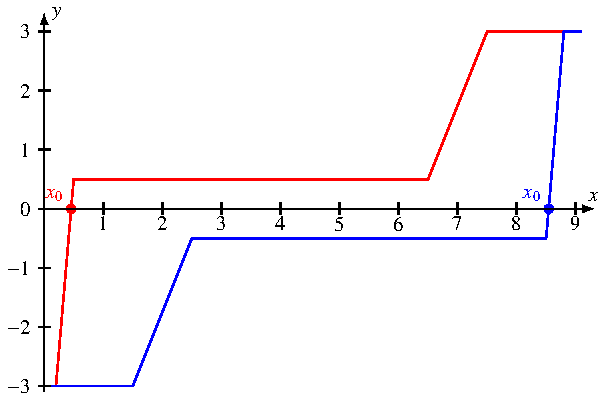
\includegraphics{chapters/20-gleichungen/figures/stufe.pdf}
\caption{Die Werte einer stetigen Funktion an den Intervallenden verraten
nichts über die Lage einer Nullstelle im Interval.
Die beiden Graphen gehören zu Funktionen, die den gleichen Wert an den
Intervallenden haben, aber die Nullstelle $x_0$ liegt an völlig
unterschiedlichen Stellen
\label{buch:figure:stufe}}
\end{figure}

Man beachte, dass der Betrag der Funktionswerte an den Intervallenden keine
Information darüber liefert, wo im Interval die Nullstelle zu finden ist.
Abbildung~\ref{buch:figure:stufe} zeigt zwei Funktionen mit identischen
Funktionswerten an den Intervallenden aber völlig verschiedener Lage
der Nullstellen.
Erst zusätzliche Annahmen über die Steigung oder Krümmung der Kurve können
die Lage der Nullstelle besser eingrenzen.

Der Zwischenwertsatz~\ref{buch:satz:nullstellenzwsatz} liefert trotzdem
genug Information, um die Nullstelle zu finden.
Für die folgende Diskussion nehmen wir der Einfachheit an, dass $f(a)<0$
und $f(b)>0$ ist.
Wir wissen bereits, dass die Nullstelle im Interval $[a,b]$ liegen muss.
Sei $m=\frac12(a+b)$ der Mittelpunkt des Intervals.
Wenn $f(m) > 0$ ist, können wir schliessen, dass eine Nullstelle im
Teilinterval $[a,m]$ liegen muss.
Wenn $f(m) <0$ ist, liegt eine Nullstelle in $[m,b]$.
Damit ist ein neues Interval halber Länge gefunden, welches eine
Nullstelle von $f$ enthält.
Durch Wiederholen dieses Prozesses können wir ein beliebige kleines
Interval erhalten, welches eine Nullstelle enthält.
Nach dem Intervalschachtelungsprinzip der Analysis definiert dies
die Nullstelle.

\begin{satz}[Intervallhalbierung]
Sei $f\colon[a,b]\to\mathbb R$ eine stetige Funktion mit $f(a)<0$ und
$f(b)>0$.
Sei $I_k=[a_k,b_k]$ die Folge von Intervallen rekursiv definiert wie folgt.
\begin{enumerate}
\item
Das Startinterval hat Intervallenden $a_0=a$ und $b_0=b$.
\item
Sei $m_k = \frac12(a_k+b_k)$.
Das Intervall $I_{k+1}$ ist 
\[
I_{k+1} = [a_{k+1},b_{k+1}] = 
\begin{cases}
[a_k,m_k]&\qquad f(m_k) > 0\\[5pt]
[m_k,b_k]&\qquad f(m_k) < 0.
\end{cases}
\]
\end{enumerate}
Die Intervalle $I_k$ haben die folgenden Eigenschaften
\begin{enumerate}
\item
Die Länge der Intervalle halbiert sich in jeder Iteration: $|I_k|=2^{-k}(b-a)$.
\item
Für jedes Intervall gilt $f(a_k)<0$ und $f(b_k)> 0$.
\item
Die Schnittmenge
$\bigcap_{k=0}^\infty I_k$ enthält nur den Wert
\[
x_0 = \lim_{k\to\infty}a_k=\lim_{k\to\infty}b_k=\lim_{k\to\infty}m_k,
\]
der eine Nullstelle der Funktion $f$ ist.
\end{enumerate}
\end{satz}

\begin{proof}[Beweis]
Es ist nur noch die Ausssage über die Konvergenz der Folgen $a_k$ und $b_k$
zu beweisen.
Da aber die Intervall-Länge $|I_k|=2^{-k}(b-a)$ ist, kann man die
Entfernung der Folgenglieder voneinander abschätzen.
Ist $k=\min\{m,n\}$, dann folgt
\[
|a_m-a_n| < 2^{-k}(b-a),\quad
|b_m-b_n| < 2^{-k}(b-a),\quad
|m_m-m_n| < 2^{-k}(b-a).
\]
Wählt man $N$ so gross, dass $2^{-N}(b-a)<\varepsilon$ ist, dann
folgt für jedes beliebige $\varepsilon>0$, dass 
\[
|a_m-a_n|<\varepsilon,\quad
|b_m-b_n|<\varepsilon,\quad
|m_m-m_n|<\varepsilon,
\]
die Folgen sind also Cauchy-Folgen.
\end{proof}

Die Konvergenzgeschwindigkeit des Intervall-Halbierungs-Verfahrens ist
sehr beschränkt.
Der Fehler halbiert sich in jeder Iteration, man gewinnt also genau
1 Bit Genauigkeit.
Für die volle Genauigkeit eines Gleitkomma-Typs der Maschine braucht
man also etwa soviele Iterationen, wie die Mantisse Binärstellen hat,
aber auch nur, wenn das erste Bit und der Exponent bereits richtig
sind.

\begin{beispiel}
Als Beispiel berechnen wir $\sqrt[100]{10}$.
Die Potenzfunktion $p(x)=x^{100}$, die wir dazu invertieren müssen, hat
extrem grosse Steigung in der Näher der Lösung.
Es muss eine Nullstelle der Funktion $f(x)=x^{100}-10$ gefunden werden.
Wegen $f(0)=-10$ und $f(2)\simeq 1.2677\cdot 10^{30}$ muss das Intervall
$[0,2]$ eine Nullstelle enthalten.
Weil die Funktion monoton wachsend ist, ist es auch die einzige.
Der Wert $f(2)$ ist klein genug für den \texttt{float} Typ,
daher kann man die Berechnung in \texttt{float} durchführen.

\begin{table}
\centering
\begin{tabular}{|>{$}r<{$}|>{$}r<{$}|>{$}r<{$}|>{$}r<{$}|}
\hline
k&a_k&b_k& b_k-a_k\\
\hline
 0 & 0.00000000 & 2.00000000 & 2.00000000\\
  1 & \color{red} \underline{1}.00000000 &             \underline{}2.00000000 & 1.00000000\\
  2 &             \underline{1}.00000000 & \color{red} \underline{1}.50000000 & 0.50000000\\
  3 &             \underline{1}.00000000 & \color{red} \underline{1}.25000000 & 0.25000000\\
  4 &             \underline{1}.00000000 & \color{red} \underline{1}.12500000 & 0.12500000\\
  5 &             \underline{1}.00000000 & \color{red} \underline{1.0}6250000 & 0.06250000\\
  6 &             \underline{1}.00000000 & \color{red} \underline{1.0}3125000 & 0.03125000\\
  7 & \color{red} \underline{1.0}1562500 &             \underline{1.0}3125000 & 0.01562500\\
  8 &             \underline{1.0}1562500 & \color{red} \underline{1.023}43750 & 0.00781250\\
  9 & \color{red} \underline{1.0}1953125 &             \underline{1.023}43750 & 0.00390625\\
 10 & \color{red} \underline{1.02}148438 &             \underline{1.023}43750 & 0.00195312\\
 11 & \color{red} \underline{1.02}246094 &             \underline{1.023}43750 & 0.00097656\\
 12 & \color{red} \underline{1.02}294922 &             \underline{1.023}43750 & 0.00048828\\
 13 & \color{red} \underline{1.023}19336 &             \underline{1.023}43750 & 0.00024414\\
 14 &             \underline{1.023}19336 & \color{red} \underline{1.023}31543 & 0.00012207\\
 15 & \color{red} \underline{1.0232}5439 &             \underline{1.023}31543 & 0.00006104\\
 16 & \color{red} \underline{1.0232}8491 &             \underline{1.023}31543 & 0.00003052\\
 17 &             \underline{1.0232}8491 & \color{red} \underline{1.023}30017 & 0.00001526\\
 18 & \color{red} \underline{1.02329}254 &             \underline{1.023}30017 & 0.00000763\\
 19 &             \underline{1.02329}254 & \color{red} \underline{1.02329}636 & 0.00000381\\
 20 &             \underline{1.02329}254 & \color{red} \underline{1.02329}445 & 0.00000191\\
 21 &             \underline{1.02329}254 & \color{red} \underline{1.023293}50 & 0.00000095\\
 22 &             \underline{1.02329}254 & \color{red} \underline{1.023293}02 & 0.00000048\\
 23 & \color{red} \underline{1.02329}278 &             \underline{1.023293}02 & 0.00000024\\
 24 & \color{red} \underline{1.023292}90 &             \underline{1.023293}02 & 0.00000012\\
\hline
\end{tabular}
\caption{Bestimmung von $\sqrt[100]{10}$ mit Hilfe des
Intervallhalbierungsverfahrens.
Die jeweils neue Intervallgrenze ist {\color{red}rot} markiert.
\label{buch:table:intervallhalbierung}}
\end{table}

Tabelle~\ref{buch:table:intervallhalbierung} zeigt den Gang der
Berechnung.
Die Implementation in C++ verwendet als Abbruchkriterium die
Länge des Intervals.
Die Iteration endet, wenn 
die Intervallänge $b_k-a_k$ den $\varepsilon$-Wert
erreicht, der für den Typ \texttt{float} im Header
\texttt{limits} definiert ist.
Wie erwartet sind soviele Iterationen nötig, wie die Mantisse 
des \texttt{float}-Typs Bits hat.

Das Programm \texttt{nullstellen.cpp}\footnote{Das Programm
kann im Verzeichnis 
\texttt{buch/chapters/experiments/nullstellen} von \cite{buch:repo}
gefunden werden.}
implementiert den Algorithmus für jeden Maschinentypen.
Damit kann man sehen, dass die berechnete Laufzeit auch für die
grösseren Gleitkommatypen durch die Bitlänge der Mantisse gegeben ist.
\end{beispiel}

\subsection{Sekanten-Verfahren
\label{buch:subsection:sekanten}}
Das Intervallhalbierungsverfahren verwendet nicht mehr als die
Stetigkeit der Funktion.
Dies führt zu sehr langsamer Konvergenz, weil die relative Grösse
der Funktionswerte in den Intervallenden keine Information über die
Lage der Nullstelle im Intervall gegen kann.
Dazu wird Information darüber benötigt, wie schnell sich Funktionswerte
ändern können.
Insbesondere muss davon ausgegangen werden können, dass die Steigung
der Funktion über das betrachtete Interval nicht zu stark schwankt.
Die Ableitung einer differenzierbaren Funktion kann diese Information
liefern, es ist aber ausreichend, eine Lipshitz-Bedingung zu verlangen,
die wie folgt definiert ist.

\begin{definition}
\label{buch:definition:lipshitz}
Die Funktion $f\colon[a,b]\to\mathbb R$ erfüllt eine Lipshitz-Bedingung
zum Exponenten $\alpha$, wenn es eine Konstante $L$ gibt derart, dass
\[
|f(x)-f(y)|
<
L|x-y|^\alpha
\]
ist.
\end{definition}

Eine Lipschitz-Bedingung limitiert, wie schnell sich der Wert
einer Funktion ändern kann.
Eine stetig differenzierbare Funktion erfüllt automatisch eine
Lipshitz-Bedingung für $\alpha=1$, die Umkehrung gilt allerdings
nicht.

Sei jetzt $f\colon[a,b]\to\mathbb R$ wieder eine Funktion mit
$f(a)<0$ und $f(b) > 0$.
Wenn $f$ eine Lipshitz-Bedingung erfüllt, dann geben die
Werte $f(a)$ und $f(b)$ zusätzlich Information über die Lage
der Nullstelle, die im Interval liegen muss.
Da sich Funktionswerte nicht beliebig schnell ändern können,
dürfte die Nullstelle näher beim kleineren Funktionswert sein.

\begin{figure}
\centering
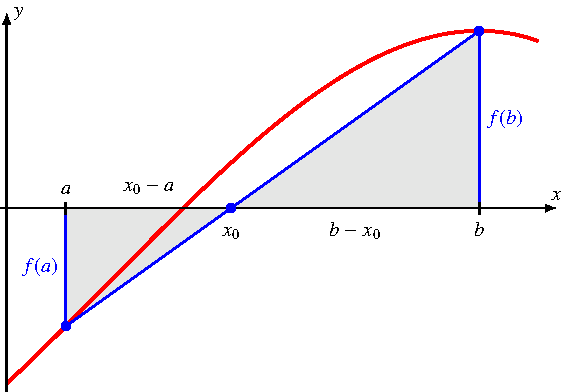
\includegraphics{chapters/20-gleichungen/figures/sekante.pdf}
\caption{Bestimmung einer neuen Schätzung $x_0$ für die Nullstelle
mit Hilfe der Sekante.
Nach dem Strahlensatz ist $(a-x_0):f(a) = (b-x_0):f(b)$, woraus
sich $x_0$ bestimmen lässt (siehe auch \eqref{buch:equation:sekante}).
\label{buch:figure:sekante}}
\end{figure}

Nehmen wir an, die Funktion $f$ sei linear zwischen den beiden
Funktionswerten, dann ist die Nullstelle der Schnittpunkt
der Geraden durch $(a,f(a))$ und $(b,f(b))$ mit der $x$-Achse.
Der Strahlensatz zeigt
\[
\begin{aligned}
&&
(a-x_0) : f(a)
&=
(b - x_0) : f(b)
\\
&\Leftrightarrow&
a\,f(b) - b\,f(a)
&=
x_0(f(b)-f(a))
\\
&\Rightarrow&
x_0
&=
\frac{a\,f(b)-b\,f(a)}{f(b)-f(a)}.
\end{aligned}
\]
Man kann diese Formel für $x_0$ auch bekommen als mit den
Funktionswerten gewichtetes Mittel der Endpunkte wie folgt.
Das Gewicht $m_a$ von $a$ ist $f(b)$, das Gewicht $m_b$ von
$b$ ist $-f(a)$, hier verwenden wir $f(a)<0$.
Das gewichtete Mittel ist dann
\begin{equation}
\frac{a\,m_a+b\,m_b}{m_a+m_b}
=
\frac{a\,f(b)-b\,f(a)}{f(b)-f(a)}=x_0.
\label{buch:equation:sekante}
\end{equation}
Indem die Intervallhalbierung durch eine Teilung des
Intervalls im Punkt $x_0$ ersetzt wird, kann ein neuer Algorithmus
gewonnen werden, der möglicherweise schneller konvergiert, weil
Intervalle schneller kleiner werden können.

Leider ist dem nicht so.
Im Intervallhalbierungsverfahren ist sichergestellt, dass das neue
Intervall hochstens halb so gross ist.
Eine solche Garantie gibt es bei Verwendung der
Formel~\eqref{buch:equation:sekante} nicht.
Ist zum Beispiel im Interval $[a,b]$ die erste Ableitung $f'(x)>0$ und
die zweite Ableitung $f''(x)<0$,
dann ist der neue Teilpunkt immer rechts von der Nullstelle.
Das neue Intervall hat daher immer den gleichen linken Endpunkt $a$,
die Folge $a_k$ konvergiert nicht.

\begin{beispiel}
Die Funktion $f(x)=\sin x - \frac12$ hat im Interval $[0,\frac{\pi}2]$
positive Steigung und negative zweite Ableitung.
Wie erwartet bleibt $a_k$ konstant, aber $b_k$ konvergiert monton
gegen die Nullstelle.
In Tabelle~\ref{buch:table:sekanten} sind die Resultate der Rechnung
gezeigt.
Die Werte der Teilpunkte $m_k$ konvergiert linear gegen den gesuchten
Wert $\arcsin\frac12$.
\begin{table}
\centering
\begin{tabular}{|>{$}r<{$}|>{$}r<{$}|}
\hline
  k & m_k \\
\hline
 -1 & 0.00000000 \\
  0 & 1.50000000 \\
  2 & \underline{0.5}5041450 \\
  3 & \underline{0.52}616811 \\
  4 & \underline{0.523}83864 \\
  5 & \underline{0.5236}2108 \\
  6 & \underline{0.5236}0088 \\
  7 & \underline{0.523598}97 \\
  8 & \underline{0.523598}79 \\
\hline
\end{tabular}
\caption{Sekanten-Verfahren zur Bestimmung von $\arcsin \frac12$.
Die Konvergenz ist unbefähr linear, aber deutlich schneller als
beim Intervallhalbierungsverfahren.
\label{buch:table:sekanten}}
\end{table}
\end{beispiel}

\begin{satz}[Sekanten-Verfahren]
Sei $f\colon[a,b]\to\mathbb R$ eine stetig Funktion mit $f(a)<0$ und $f(b)>0$,
die eine Lipshitz-Bedingung mit $\alpha=1$ erfüllt.
Setzt man $x_{-1}=a$ und $x_0=b$ und konstruiert die Folge
\[
x_{n+1} = \frac{x_{n-1}f(x_n) - x_nf(x_{n-1})}{f(x_{n})-f(x_{n-1})}.
\]
Falls $a$ und $b$ nahe genug bei einer Nullstelle der Funktion $f$ ist,
dann konvergiert die Folge $x_{n+1}$ gegen die Nullstelle.
\end{satz}

\begin{proof}[Beweis]
TODO
\end{proof}

Man beachte, dass die Bedingung an die Vorzeichen von $f(a)$ und $f(b)$
nur dazu dient, die Existenz einer Nullstelle im Intervall zu garantieren.
Ein anderes Problem dieses Verfahrens ist, dass mit genauer werdender
Approximation $x_n$ der Nullstelle die Werte $f(x_n)$ und $f(x_{n-1})$
sehr nahe beeinander liegen und damit die Differenz stark von 
Auslöschung betroffen sein wird.
Im Intervallhalbierungsalgorithmus ist dies kein Problem, weil keine
Differenzen von Funktionswerten gebildet werden und ausschliesslich das
Vorzeichen des Funktionswertes verwendet wird.




%
% newton.tex
%
% (c) 2020 Prof Dr Andreas Müller, Hochschule Rapperswil
%
\section{Newton-Verfahren
\label{buch:section:newtion}}
\rhead{Newton-Verfahren}
\index{Newton-Verfahren}%
Die bisher vorgestellten Verfahren zur Bestimmung einer Nullstelle
$x^*$ der Funktion $f$, $f(x^*)=0$ sind linear konvergent und damit
eher langsam.
\index{Nullstelle}%
Dafür war nicht mehr als Stetigkeit nötig, um Konvergenz des Verfahrens
sicherzustellen.

%
% Analytischer Ansatz
%
\subsection{Analytischer Ansatz für ein quadratisch konvergentes Verfahren
\label{buch:subsection:newton:analytisch}}
In Abschnitt~\ref{buch:subsection:linearekonvergenz} wurde dargestellt,
dass nach Möglichkeit quadratische Konvergenz angestrebt werden sollte.
\index{quadratische!Konvergenz}%
\index{Konvergenz!quadratisch}%
Quadratische Konvergenz könnte in einer Fixpunktiteration $x_{n+1}=g(x_n)$
erreicht werden, wenn die Ableitung $g'(x^*)=0$ ist.
\index{Fixpunkt}%

Je grösser $f(x_n)$ ist, desto weiter dürfte $x_n$ von der Nullstelle
entfernt sein.
Wir versuchen daher, die Approximation $x_{n+}$ proportional zum Wert von
$f(x_n)$ zu korrigieren mit Hilfe der Funktion
\[
x_{n+1} = g(x_n) = x_n - a(x_n)\cdot f(x_n).
\]
Die Funktion $a(x_n)$ muss noch bestimmt werden.
Sie soll so gewählt werden, dass die Konvergenz quadratisch wird, was
mit $g'(x^*)=0$ erreicht wird.

Die Ableitung von $g$ ist
\begin{align*}
g'(x)
&=
1-a'(x)f(x)-a(x)f'(x).
\intertext{An der Stelle $x^*$ gilt}
g'(x^*)
&=
1-a'(x^*)\underbrace{f(x^*)}_{\displaystyle=0} - a(x^*)f'(x^*) = 0
\\
\Leftrightarrow\qquad
1
&=
a(x^*) f'(x^*)
\qquad\Rightarrow\qquad
a(x)=\frac{1}{f'(x)}.
\end{align*}
Damit finden wir das im folgenden Satz beschriebene Verfahren mit
quadratischer Konvergenz.

\begin{satz}[Newton-Verfahren]
\index{Newton-Verfahren}%
\label{buch:satz:newton-verfahren}
Hat die differenzierbare Funktion $f$ eine Nullstelle $x^*$ und gilt
$f'(x^*)\ne 0$, dann konvergiert die Iterationsfolge
\begin{equation}
x_{n+1} = x_n - \frac{f(x_n)}{f'(x_n)} 
\label{buch:equation:newtoniteration}
\end{equation}
für Startwerte $x_0$ genügend nahe bei $x^*$ quadratisch gegen die
Nullstelle.
\end{satz}
\index{Startwert}%

Das Sekantenverfahren hat darunter gelitten, dass die Berechnung
der der nächsten Approximation mit Hilfe der Formel 
\eqref{buch:eqn:sekanten-iteration} von umso stärker Auslöschung
geplagt ist, je näher man bereits an der Lösung ist.
\index{Sekantenverfahren}%
Die Iterationsformel
\eqref{buch:equation:newtoniteration}
für die Newton-Iteration hat dieses Problem nicht.
In \eqref{buch:equation:newtoniteration} wird der aktuelle Wert $x_n$
um einen Korrekturbetrag korrigiert, der proportional zu $f(x_n)$
verkleinert wird.
Je genauer der Wert $x_n$ schon ist, desto kleiner wird auch die
Korrektur.

%
% Geometrische Interpretation
%
\subsection{Geometrische Interpretation des Newton-Verfahrens}
\begin{figure}
\centering
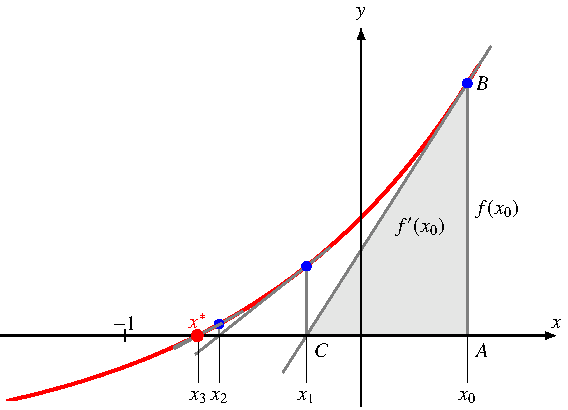
\includegraphics{chapters/20-gleichungen/figures/newton.pdf}
\caption{Graphische Interpretation des Newton-Verfahrens.
In jedem Iterationsschritt wird die bisherige Approximation $A$
mit Hilfe einer Tangente vom Funktionswert $B$ zum Punkt $C$
korrigiert, $\overline{AC}=f(x_0)/f'(x_0)$.
\label{buch:figure:newton}}
\end{figure}
Die Iterationsformel~\eqref{buch:equation:newtoniteration}
lässt sich sehr schön graphisch interpretieren.
In Abbildung~\ref{buch:figure:newton} wird die Nullstelle der
Funktion $f(x) = e^x-\frac12$ mit dem Newton-Verfahren bestimmt.
Im Iterationsschritt wird die Approximation $x_n$ korrigiert
nach der Formel
\[
x_{n+1}
=
x_n - \frac{f(x_n)}{f'(x_n)}
=
x_n - \frac{e^{x_n}-\frac12}{e^{x_n}}
=
x_n - \biggl(1 -\frac{e^{-x_n}}{2}\biggr)
\]
Die Korrektur für $n=0$ ist in Abbildung~\ref{buch:figure:newton}
als Grundseite des rechtwinkligen Dreiecks $ABC$ erkennbar.
Die Hypothenuse hat die Steigung $f'(x_0)$, daher ist
\index{Hypothenuse}%
\index{Dreieck}%
\[
\overline{AC}\cdot f'(x_0) = f(x_0)
\qquad\Rightarrow\qquad
\overline{AC} = \frac{f(x_0)}{f'(x_0)}.
\]
Die vom Newton-Verfahren berechnete Korrektur ist also die optimale
Korrektur, die sich aus Funktionswert und erster Ableitung
an der Stelle $x_n$ berechnen lässt.
\index{Ableitung}%

%
% Wurzeln
%
\subsection{Wurzeln}
Als Beispiel für die Anwendung des Newton-Verfahrens berechnen wir die
$k$-te Wurzel einer positiven reellen
Zahl $a$, wir lösen also die Gleichung
$x^k = a$.
\index{Wurzel}%
Dies ist gleichbedeutend damit, eine Nullstelle der Funktion
$f(x)=x^k-a$ zu bestimmen.
Die Ableitung von $f$ ist
$f'(x)=kx^{k-1}$, woraus wir die Iterationsformel des
Newton-Verfahrens ablesen können:
\[
x_{n+1} = x_n - \frac{f(x_n)}{f'(x_n)}=x_n - \frac{x_n^k-a}{kx_n^{k-1}}
=
\frac{1}{k}\biggl((k-1)x_n+\frac{a}{x_n^{k-1}}\biggr).
\]
Im Falle $n=2$ finden wir das bereits in 
Abschnitt~\ref{buch:subsection:linearekonvergenz}
untersuchte, quadratisch konvergente Verfahren zur Bestimmung
der Quadratwurzel wieder.
\index{Quadratwurzel}%
In Tabelle~\ref{buch:table:wurzel5newton} ist das Verfahren für
$a=10$, $k=5$ und $x_0=a$ gezeigt.
Quadratische Konvergenz stellt sich allerdings erst bei $x_{10}$ ein,
der Startwert $x_0$ ist zu weit von der Lösung entfernt.

\begin{table}
\centering
\renewcommand\arraystretch{1.15}
\begin{tabular}{|>{$}r<{$}|>{$}r<{$}|}
\hline
n& x_n\\
\hline
 0 & 10.00000000000000\\
 1 &  8.00020000000000\\
 2 &  6.40064823242493\\
 3 &  5.12171019598693\\
 4 &  4.10027465454472\\
 5 &  3.28729556684556\\
 6 &  2.64696320430731\\
 7 &  2.15831219143923\\
 8 &  \underline{1}.81881622015378\\
 9 &  \underline{1.}63781027109793\\
10 &  \underline{1.58}820394873794\\
11 &  \underline{1.5849}0696686523\\
12 &  \underline{1.584893192}70054\\
13 &  \underline{1.58489319246111}\\
\hline
\infty&\sqrt[5]{10}=1.58489319246111\\
\hline
\end{tabular}
\caption{Berechnung von $\sqrt[5]{10}$ mit dem Newton-Verfahren.
Der Startwert $x_0=10$ ist sehr weit von der Lösung entfernt, so dass es
einige Iterationen braucht, bis die Konvergenz quadratisch wird.
\label{buch:table:wurzel5newton}}
\end{table}

%
% Newton-Verfahren in R^n
%
\subsection{Newton-Verfahren in $\mathbb R^n$
\label{buch:section:newtoninRn}}
\index{Newton-Verfahren!in $\mathbb R^n$}%
In der bisher beschriebenen Form erlaubt das Newton-Verfahren, 
Nullstellen von rellwertigen Funktion zu finden.
Es eignet sich nicht, Vektorgleichungen zu lösen.
\index{Vektorgleichung}%

Sei daher im folgenden $f\colon \mathbb R^k \to \mathbb R^k$ eine
Vektorfunktion mit einer Nullstelle $x^*$, $f(x^*)=0$, die numerisch gefunden 
werden soll.
Wie in Abschnitt~\ref{buch:subsection:newton:analytisch} soll eine
Approximation $x_n$ für die Nullstelle $x^*$ proportional zur Grösse
von $f(x_n)$ korrigiert werden.
Eine skalare Funktion $a(x)$ wird aber im allgemeinen zu wenig
allgemein für eine performante Lösung des Problem sein, daher
wird für $A(x)$ eine matrixwertige Funktion mit Werten in
$\operatorname{GL}_k(\mathbb R)$ gewählt.
\index{Funktion!matrixwertig}%
\index{GLkR@$\operatorname{GL}_k(\mathbb R)$}%
Wir setzen also an
\[
x_{n+1} = g(x_n) = x_n - A(x_n) f(x_n)
\]
und versuchen wie früher $A(x)$ so zu wählen, dass die Ableitung von $g$
an der Stelle $x^*$ verschwindet.

Die Ableitung von $g(x)=x-A(x)f(x)$ ist
eine lineare Abbildung, die auf dem Vektor $h\in\mathbb R^k$ den Wert
\begin{align*}
Dg(x) \cdot h
&=
h - (DA(x)\cdot h) f(x) - A(x) Df(x)\cdot h
\end{align*}
hat.
An der Stelle $x=x^*$ verschwindet der mittlere Term wegen $f(x^*)=0$, so
dass als Gleichung für $A(x)$
\[
0=h-A(x) Df(x) \cdot h
\qquad\Rightarrow\qquad
h = A(x) Df(x) \cdot h\qquad \forall h\in\mathbb R^n
\]
übrigbleibt.
Dies ist nur möglich, wenn $A(x)$ die inverse Matrix von $Df(x)$ ist,
was den folgenden Satz motiviert.

\begin{satz}[Newton-Verfahren für Vektorgleichungen]
\label{buch:satz:newtonVektorgleichungen}
\index{Newton-Verfahren!für Vektorgleichungen}%
Hat die Funktion $f\colon\mathbb R^k\to\mathbb R^k$ eine Nullstelle
$x^*\in\mathbb R^n$, dann ist die Folge 
\[
x_{n+1} = x_n - Df(x_n)^{-1}\cdot f(x_n)
\]
für Startwerte $x_0$ nahe genug an $x^*$ quadratisch konvergent mit
Grenzwert $x^*$.
\end{satz}

\begin{proof}[Beweis]
Es ist klar, das $x^*$ ein Fixpunkt der Abbildung
\[
g(x)=x-Df(x)^{-1}\cdot f(x)
\]
ist.
Wir müssen nur noch zeigen, dass der Fehler der Iteration quadratisch
abnimmt.
Dazu entwickeln wir $f$ um den Punkt $x^*$ in eine Taylor-Reihe
\begin{align*}
f(x^* + \delta)
&=
f(x^*) + Df(x^*)\cdot \delta + O(|\delta|^2),\qquad\delta\in\mathbb R^k
\\
&=
Df(x^*)\cdot \delta + O(|\delta|^2)
\end{align*}
wegen $f(x^*)=0$.
Die Iteration ist
\begin{align}
x_{n+1}
&=
x^* +\delta_{n+1}
=
g(x^*+\delta_n)
=
x^*+\delta_n  - Df(x_n)^{-1}\cdot f(x_n)
\notag
\\
&=
x^* + \delta_n -Df(x_n)^{-1}\cdot f(x^* + \delta_n)
\notag
\\
&=
x^* + \delta_n -Df(x_n)^{-1}\cdot
(Df(x^*)\cdot \delta_n + O(|\delta_n|^2).
\label{buch:equation:newtonn:iteration}
\end{align}
Um \eqref{buch:equation:newtonn:iteration}
zu berechnen, muss man auch $Df(x_n)$ in eine Taylor-Reihe entwickeln, sie ist
\index{Taylor-Reihe}%
\[
Df(x_n)
=
Df(x^*+\delta_n)
=
Df(x^*) + D^2f(x^*)\cdot\delta_n.
\]
Setzt man dies in~\eqref{buch:equation:newtonn:iteration} ein, erhält man
\begin{align*}
x_{n+1}
=
x^*+\delta_{n+1}
&=
x^* + \delta_n -
(Df(x^*) + D^2f(x^*)\cdot\delta_n)^{-1}
(Df(x^*)\cdot \delta_n + O(|\delta_n|^2)
\\
&=
x^* + \delta_n -
(Df(x^*)^{-1} + O(|\delta_n|))
\cdot
(Df(x^*)\cdot \delta_n + O(|\delta_n|^2)
\\
&=
x^* + \delta_n
- \underbrace{Df(x^*)^{-1}Df(x^*)}_{\displaystyle = E}\mathstrut\cdot\delta_n
+
O(|\delta_n|^2)
\\
&=x^* + O(|\delta_n|^2).
\end{align*}
Der Fehler $\delta_{n+1}=O(|\delta_n|^2)$ nimmt somit quadratisch ab
und damit ist gezeigt, dass die Iterationsfolge quadratrisch
konvergiert.
\index{Iterationsfolge}%
\end{proof}

\begin{beispiel}
Es sollen die Polarkoordinaten des Punktes $(x,y)$
\index{Polarkoordinaten}%
als Lösung der Gleichung
\[
\begin{pmatrix}
r\cos\varphi\\r\sin\varphi
\end{pmatrix}
=
\begin{pmatrix}x\\y\end{pmatrix}
\qquad\Rightarrow\qquad
f(r,\varphi) =\begin{pmatrix}r\cos\varphi -x \\ r\sin\varphi -y \end{pmatrix}
=0
\]
bestimmt werden.
Dies ist ein Beispiel für die Dimension $k=2$.

Die Ableitungsmatrix von $f$ ist
\index{Ableitungsmatrix}%
\[
Df(r,\varphi)
=
\begin{pmatrix}
\cos\varphi&-r \sin\varphi\\
\sin\varphi&\phantom{-} r \cos\varphi
\end{pmatrix}
\qquad\Rightarrow\qquad
Df(r,\varphi)^{-1}
=
\begin{pmatrix}
\cos\varphi&\sin\varphi\\
-\frac1r\sin\varphi&\frac1r\cos\varphi
\end{pmatrix}.
\]
Die Iterationsformel wird jetzt
\begin{align}
\begin{pmatrix}
r_{n+1}\\
\varphi_{n+1}
\end{pmatrix}
&=
\begin{pmatrix}r_n\\\varphi_n\end{pmatrix}
-
\begin{pmatrix}
\cos\varphi_n&\sin\varphi_n\\
-\frac1{r_n}\sin\varphi_n&\frac1{r_n}\cos\varphi_n
\end{pmatrix}
\begin{pmatrix}
r_n\cos\varphi_n-x\\
r_n\sin\varphi_n-y
\end{pmatrix}
\notag
\\
&=
\begin{pmatrix}
x\cos\varphi_n+y\sin\varphi_n\\
\varphi_n -\frac{x}{r_n}\sin\varphi_n+\frac{y}{r_n}\cos\varphi_n
\end{pmatrix}
\label{buch:equation:polar}
\end{align}
\begin{table}
\centering
\begin{tabular}{|>{$}r<{$}|>{$}r<{$}>{$}r<{$}|}
\hline
n &                r_n               &                    \varphi_n    \\
\hline
0 &              3.1415926535897931  &              0.3678794411714423 \\
1 &              0.8067763763745672  &              0.5559550343664228 \\
2 &   \underline{0.9}030213557712843 &   \underline{1.0}884392177149671 \\
3 &   \underline{0.99}60918007116625 &   \underline{0.99}06298199545209 \\
4 &   \underline{0.9999}561001841604 &   \underline{1.0000}366265580796 \\
5 &   \underline{0.999999999}3292477 &   \underline{0.99999999}83920385 \\
6 &   \underline{1.0000000000000000} &   \underline{1.0000000000000000} \\
\hline
\infty& 1.0000000000000000 &   1.0000000000000000 \\
\hline
\end{tabular}
\caption{Quadratische Konvergenz des Iterationsverfahrens
\eqref{buch:equation:polar}
zur Bestimmung der Polarkoordinaten 
\label{buch:figure:newtonpolar}}
\end{table}%
Die Resultate der Iteration~\eqref{buch:equation:polar} für 
den Punkt $(x,y)=(\cos 1,\sin 1)$ ist in 
Tabelle~\ref{buch:figure:newtonpolar} gegeben.
Die quadratische Konvergenz ist wieder deutlich erkennbar.
\end{beispiel}

%
% Der Fahll f'(x)=0
%
\subsection{Der Fall $f'(x^*)=0$
\label{buch:subsection:newton0}}
Im Fall $f'(x^*)=0$ versagt die Iterationsformel des Newton-Verfahrens.
Es ist damit zu rechnen, dass das Verfahren sehr langsam oder gar nicht
konvergiert.
Wir untersuchen dies mit Hilfe einer Entwicklung der Funktion $f$
um den Punkt $x^*$:
\[
f(x^*+\delta)
=
x^*
+
\frac12f''(x^*)\delta^2 + \frac16f'''(x^*)\delta^3+ O(\delta^4).
\]
Für den Fehler $\delta_n$ der Approximation $x_n=x^*+\delta_n$ folgt die
Iteration
\begin{align*}
x^*+\delta_{n+1}
=
x_{n+1}
&=
x_n - \frac{f(x_n)}{f'(x_n)}
=
x^*+\delta_n
-
\frac{
\frac12f''(x^*)\delta_n^2+O(\delta_n^4)
}{
f''(x^*)\delta_n + \frac12f'''(x^*)\delta_n^2) + O(\delta^3)
}
\\
&=
x^* + \delta_n
-
\frac12
\delta_n
\frac{1+O(\delta_n)}{1+O(\delta_n)}
=
x^* + \delta_n
-
\frac12
\delta_n
(1+O(\delta_n))
\\
&=
x^* +\frac12\delta_n + O(\delta_n^2)
\\
\Rightarrow\qquad
\delta_{n+1} &= \frac12\delta_n + O(\delta_n^2)
\end{align*}
Der Fehler halbiert sich in jeder Interation.
Die Folge $(x_n)_{n\in\mathbb N}$ konvergiert also immer noch,
aber die Konvergenz ist nur noch linear.

%
% Vergleich mit dem Sekantenverfahren
%
\subsection{Vergleich mit dem Sekantenverfahren
\label{buch:subsection:newtonsekanten}}
\index{Sekantenverfahren}%
Die Ähnlichkeit des Newton-Verfahrens mit dem Sekantenverfahren ist 
unübersehbar.
Um dies deutlich zu machen, berechnen wir den Grenzfall $x_{n-1}\to x_n$
mit Hilfe der Form~\eqref{buch:sekante:stabil}.
%\begin{align*}
%x_{n+1}
%&=
%\frac{x_{n-1}f(x_n)-x_nf(x_{n-1})}{f(x_{n})-f(x_{n-1})}
%=
%\frac{x_{n-1}f(x_n){\color{darkred}\mathstrut-x_{n-1}f(x_{n-1})+x_{n-1}f(x_{n-1})}-x_nf(x_{n-1})}{f(x_{n})-f(x_{n-1})}
%\\
%&=
%x_{n-1} - f(x_{n-1})\frac{x_n-x_{n-1}}{f(x_n)-f(x_{n-1})}.
%\intertext{
Beim Grenzübergang $x_{n-1}\to x_n$ geht der Quotient auf der rechten
Seite in den Kehrwert der Ableitung $f'(x_n)$ über.
\index{Grenzübergang}%
Der Grenzfall des Sekantenverfahrens ist daher
%}
\begin{align*}
x_{n+1}
&=
x_n -\frac{f(x_n)}{f'(x_n)},
\end{align*}
also das Newton-Verfahren.
\index{Newton-Verfahren}%

Der Vorteil des Newton-Verfahrens gegenüber dem Sekantenverfahren ist
jedoch, dass die Ableitung nicht nur mit Hilfe eines Differenzenquotienten
approximiert wird, sondern exakt zur Verfügung steht.
Damit ist das Newton-Verfahren nicht anfällig auf die Auslöschung, die
die Zuverlässigkeit des Sekantenverfahrens beeinträchtigt.

%
% Nullstellen on Polynomen
%
\subsection{Nullstellen von Polynomen
\label{buch:subsection:polynomnullstellen}}
\index{Polynom}%
\index{Polynom!Nullstellen}%
Das Newton-Verfahren verlang, dass die Ableitung $f'(x_n)$ genau
berechnet werden kann.
In einigen Fällen kann dies ein Hindernis für die Anwendung des
Verfahrens sein.
Polynome sind jedoch einfach genug, dass die Ableitung immer berechnet
werden kann.
\index{Ableitung}%
Somit ist das Newton-Verfahren besonders gut geeignet, Nullstellen von
Polynomen zu finden.
In diesem Abschnitt sei daher
\begin{equation}
f(X) = a_nX^n + a_{n-1}X^{n-1} + \dots + a_2X^2 + a_1X + a_0
\label{buch:equation:nullstellenpolynom}
\end{equation}
ein Polynom mit reellen Koeffizienten, $a_k\in\mathbb R$.
Wir gehen davon aus, dass $f$ eine reelle Nullstelle $x^*$ hat
und dass $x_0$ eine ausreichend genaue Schätzung für die Nullstelle ist.

\subsubsection{Berechnung von Funktionswerten}
Die übliche Darstellung~\eqref{buch:equation:nullstellenpolynom}
ist nicht die effizienteste Form zur Berechnung des Polynomwertes.
Die Berechnung der Potenzen $x^k$ für $1\le k\le n$ benötigt bereits
$n-1$ Multiplikationen, dazu kommen $n-1$ Multiplikationen mit
Koeffizienten und $n$ Additionen.
Zudem besteht die Gefahr von Verschmierung.

Durch Ausklammern möglichst vieler Faktoren $x$ findet man die
Formel
\index{Ausklammern}%
\begin{align}
f(x)
&=
((\dots((a_nx+a_{n-1})x+a_{n-2})x+\dots)x+a_1)x+a_0,
\label{buch:equation:polynomwert}
\end{align}
welche den Funktionswert in genau $n$ Multiplikationen und $n$ Additionen
zu berechnen gestattet.

Wir bezeichnen die Teilprodukte in \eqref{buch:equation:polynomwert} mit
\index{Teilprodukte}%
\[
(\dots((a_nx+a_{n-1})x+a_{n-2})x+\dots)x+a_k
=
p_{n-k},
\]
d.~h.
\begin{equation}
\begin{aligned}
p_0 &= a_n
\\
p_1 &= a_nx+a_{n-1} = p_0x + a_{n-1}
\\
p_2 &= (a_nx+a_{n-1})x+a_{n-2} = p_1x+a_{n-2}
\\
\vdots\;&\qquad\vdots
\\
f(x)
=
p_n
&=
p_{n-1}x+a_0.
\end{aligned}
\label{buch:equation:reste}
\end{equation}
Diese Berechnung lässt sich in der folgenden, {\em Horner-Schema}
genannten Tabelle
\index{Horner-Schema}%
zusammenfassen.
\begin{center}
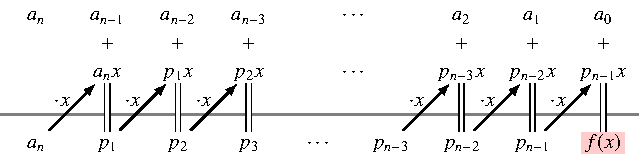
\includegraphics{chapters/20-gleichungen/figures/horner1.pdf}
\end{center}

\begin{beispiel}
Wir berechnen den Wert des Polyoms
\[
f(X) = X^6 - X^5 + X^4 - X^3 + X^2 - X + 1
\]
an der Stelle $X=2$ mit Hilfe des Horner-Schemas
\begin{center}
\begin{tabular}{>{$}r<{$}>{$}r<{$}>{$}r<{$}>{$}r<{$}>{$}r<{$}>{$}r<{$}>{$}r<{$}}
 1& -1& 1& -1&  1& -1&  1\\
  &  2& 2&  6& 10& 22& 42\\
\hline
 1&  1& 3&  5& 11& 21& 43
\end{tabular}
\end{center}
Der Wert in der rechten unteren Ecke stimmt überein mit
\begin{align*}
f(2)
&=
2^6-2^5+2^4-2^3+2^2-2+1
\\
&=
64-32+16-8+4-2+1
\\
&=
32+8+2+1
=
43.
\qedhere
\end{align*}
\end{beispiel}

\subsubsection{Deflation}
Die Bedeutung der Werte $p_0,\dots,p_{n-1}$ lässt sich verstehen, wenn
man den Polynomdivisionsalgorithmus für $f(X) / (X-x)$ ausschreibt.
\index{Polynomdivision}%
Die Rekursionsformeln~\eqref{buch:equation:reste} zeigen, dass die
Teilreste der Division die Koeffizienten $p_k$ haben:
\index{Division}%
\index{Teilreste}%
\begin{equation}
\setcounter{MaxMatrixCols}{20}
\setlength\arraycolsep{1pt}
\renewcommand\arraystretch{1.15}
\begin{matrix}
(a_nX^n&+&a_{n-1}X^{n-1}&+&a_{n-2}X^{n-2}&+&a_{n-3}X^{n-3}&+&\dots)&:&(X&-&x)&=&a_nX^{n-1}+p_1X^{n-2}+p_2X^{n-3}+\dots\\
 a_nX^n&-&a_{n}xX^{n-1} & &              & &              & &      & &  & &  & &                \\
\cline{1-3}
       & &p_1X^{n-1}    &+&a_{n-2}X^{n-2}& &              & &      & &  & &  & &                \\
       & &p_1X^{n-1}    &-&p_1xX^{n-2}   & &              & &      & &  & &  & &                \\
\cline{3-5}
       & &              & &p_2X^{n-2}    &+&a_{n-3}X^{n-3}& &      & &  & &  & &\\
       & &              & &p_2X^{n-2}    &-&a_{n-4}xX^{n-3}&&      & &  & &  &\\
\cline{5-7}
       & &              & &              & &p_3X^{n-3}     &&\dots & &  & &  &\\
       & &              & &              & &\dots          &&\dots & &  & &  &\\
\end{matrix}
\end{equation}
Die Koeffizienten $p_k$ sind daher auch die Koeffizienten des Quotienten
\[
q(X)
=
p_0X^{n-1}+p_1X^{n-2}+p_2X^{n-3}+\dots p_{n-2}X+p_{n-1}.
\]
Es gilt daher
\[
f(X)
=
(X-x) \cdot (p_0X^{n-1}+p_1X^{n-2}+p_2X^{n-3}+\dots p_{n-2}X+p_{n-1})
+
f(x).
\]
Ist $x$ ein Nullstelle, dann ist das Polynom ist $f(X)$ durch $X-x$ teilbar
und $q(X)$ ist der andere Faktor, also $f(X)=(X-x)\cdot q(X)$.
Das Polynom $q(X)$ hat Grad $n-1$, die Suche nach weiteren Nullstellen
wird also vereinfacht. 
Man nennt den Prozess, eine Nullstelle aus dem Polynom $f(X)$
herauszudividieren, {\em Deflation}.
\index{Nullstelle}%
\index{Deflation}%

\begin{beispiel}
Das Polynom
\[
f(x)=x^4-25x^2+144
\]
hat eine Nullstelle $x=3$ und $x=4$ als Nulllstellen.
Man finde zwei weitere Nullstellen.

Die Polynomdivision mit dem Horner-Schema für $x=3$
\begin{center}
\begin{tabular}{>{$}r<{$}>{$}r<{$}>{$}r<{$}>{$}r<{$}>{$}r<{$}}
   1&   0& -25&   0& 144\\
    &   3&   9& -48&-144\\
\hline
   1&   3& -16& -48&   0
\end{tabular}
\end{center}
ergibt 
\[
q_1(x) = f(x)/(x-3)
=
x^3+3x^2-16x-48
.
\]
Weiter bekommt man
\[
a_2(x) = f(x)/((x-3)(x-4)) = (x^2+7x+12) = (x+3)(x+4)
\]
aus
\begin{center}
\begin{tabular}{>{$}r<{$}>{$}r<{$}>{$}r<{$}>{$}r<{$}}
   1&   3& -16& -48\\
    &   4&  28&  48\\
\hline
   1&   7&  12&   0
\end{tabular}
\end{center}
Insbesondere schliesst man, dass $x=-3$ und $x=-4$ die verbleibenden
Nullstellen von $f(x)=(x-3)(x-4)(x+4)(x+3)$ sind.
\end{beispiel}


\subsubsection{Berechnung der Ableitung}
\index{Ableitung eines Polynoms}%
Für das Newton-Verfahren wird ausser dem Funktionswert auch die Ableitung
benötigt.
Der Funktionswert $r=f(x)$ wird mit dem Horner-Schema sofort gefunden, ebenso
\index{Horner-Schema}%
der Quotient $q(x)$,
Es gilt also
\[
f(X) = q(X)(X-x) + r,
\]
was wir dazu verwenden können, die Ableitung von $f$ mit Hilfe der
Produktregel zu berechnen:
\index{Produktregel}%
\[
f'(X) = q'(X) (X-x) + q(X).
\]
An der Stelle $X=x$ ist daher
$ f'(x) = q(x) $.
Da die Koeffizienten von $q(X)$ bereits mit dem Horner-Schema
berechnet worden sind, kann $f'(x)$ durch Iteration des Horner-Schemas
berechnet werden.

\begin{beispiel}
Man berechne den Funktionswert und die Ableitung des Polynoms
\[
f(x) = 2x^3 + x + 9
\]
an der Stelle $x=4$.
Zweimalige Anwendung des Horner-Schemas ergibt
\begin{center}
\begin{tabular}{>{$}r<{$}>{$}r<{$}>{$}r<{$}>{$}r<{$}}
   2&   0&   1&   9\\
    &   8&  32& 132\\
\hline
   2&   8&  33& 141\\
    &   8&  64&    \\
\hline
   2&  16&  97&
\end{tabular}
\end{center}
Man liest $f(4)=141$ und $f'(4)=97$ ab.
\end{beispiel}

Ist $x$ eine doppelte Nullstelle des Polynoms $f(x)$, dann ist $f'(x)=0$.
\index{Nullstelle!doppelte}%
\index{doppelte Nullstelle}%
Das Horner-Schema kann daher auch dazu verwendet werden, doppelte
Nullstellen zu erkennen und damit die Faktorisierung zu vereinfachen,
wie das folgende Beispiel zeigt.
\index{Faktorisierung}%

\begin{beispiel}
Wir betrachten das Polynom
\[
f(x) = x^4-13x^3 +41x^2 - 47x+18.
\]
Es hat die Nullstelle $x=1$, das Horner-Schema liefert für den Quotienten
\begin{center}
\begin{tabular}{>{$}r<{$}>{$}r<{$}>{$}r<{$}>{$}r<{$}>{$}r<{$}}
 1&-13& 41&-47& 18\\
  &  1&-12& 29&-18\\
\hline
 1&-12& 29&-18&  0\\
  &  1&-11& 18&   \\
\hline
 1&-11& 18&  0&   \\
  &  1&-10&   &   \\
\hline
 1&-10&  8&   &   
\end{tabular}
\end{center}
Daraus kann man ablesen, dass $x=1$ eine doppelte aber nicht
eine dreifache Nullstelle ist und dass sich das Polynom schreiben lässt als
\[
f(x)=(x-1)^2\cdot (x-11x+18) = (x-1)^2 (x-2)(x-9).
\]
Damit ist das Polynom $f(x)$ vollständig faktorisiert.
\end{beispiel}

\subsubsection{Newton-Verfahren für Nullstellen von Polynomen}
Da mit dem Horner-Schema sowohl Funktionswerte wie auch Ableitungen
effizient berechnet werden können, kann es dazu verwendet werden,
das Newton-Verfahren für Polynomnullstellen zu implementieren.

Das Horner-Schemas liefert zu jeder Nullstelle $x$ auch immer
gleich den Quotienten $q(X)=f(X)/(X-x)$, welches für die Suche nach
weiteren Nullstellen verwendet werden kann (Deflation).
\index{Deflation}%

\begin{beispiel}
\begin{table}
\centering
\renewcommand\arraystretch{1.15}
\begin{tabular}{|>{$}r<{$}|>{$}r<{$}|>{$}r<{$}|>{$}r<{$}|>{$}l<{$}|}
\hline
n& x_n & f(x_n) & f'(x_n) & q_n(X) \\
\hline
0&-10.000000& -182.00000&129.00000& X^2-X+19\\
1&- \underline{8}.589148&  -38.99232& 75.71571& X^2+0.4108524323 X+5.47112751\\
2& -\underline{8.0}74164&   -4.31028& 59.24143& X^2+0.9258356094 X+1.524651051\\
3& -\underline{8.00}1407&   -0.08021& 57.04221& X^2+0.9985933304 X+1.009848595\\
4& -\underline{8.000000}&   -0.00005& 57.00003& X^2+0.9999990463 X+1.000006676\\
5& -\underline{8.000000}&    0.00000& 57.00000& X^2+X+1\\
\hline
\end{tabular}
\caption{Newton-Verfahren für das Polynom $f(X)=X^3+9X^2+9X+8$
mit Hilfe des Horner-Schemas.
Als Nebeneffekt bestimmt das Horner-Schema in jeder Iteration auch
den Quotienten $q_n(x)=f(x)/(x-x_n)$.
\label{buch:table:hornernewton}}
\end{table}
Die reellen Nullstellen
von $f(X)=X^3+9X^2+9X +8$ sollen mit Hilfe des
Newton-Verfahrens gefunden werden.
Die Tabelle~\ref{buch:table:hornernewton} zeigt die vom Horner-Schema
berechneten Funktions- und Ableitungswerte sowie das Quotientenpolynom.
\index{Quotient!Polynom}%
Die Konvergenz ist quadratisch und liefert die Nullstelle $x=-8$
sowie den Quotienten $q(X)=X^2+X+1$,
tatsächlich ist
\[
(X+8)q(X) = (X+8)(X^2+X+1) = X^3+9X^2+9X+8 = f(X).
\]
Die Diskriminante von $q(X)$ ist
$b^2-4ac= 1^2 -4\cdot1\cdot 1= - 3<0$, $q(X)$ hat also keine weiteren
reellen Nullstellen.
\end{beispiel}

%
% normalverteilung.tex
%
% (c) 2020 Prof Dr Andreas Müller, Hochschule Rapeprswil
%
\subsection{Inverse der Normalverteilungsfunktion
\label{buch:subsection:inversenormal}}
Das Integral der Standardnormalverteilungsdichte
\[
\Phi(x) = \int_{-\infty}^x e^{-t^2/2}\,dt
\]
kann nicht in geschlossener Form berechnet werden und erst recht
nicht invertiert werden.
Für die Anwendung wird jedoch die Umkehrfunktion benötigt, zu einem Wert
$p\in[0,1]$ ist dasjenige $x$ zu finden, für welches $F(x)=p$ gilt.
Im Beispiel auf Seite~\pageref{buch:beispiel:erfc} wurde gezeigt,
wie die Fehlerfunktion
\[
\operatorname{erf}(x) = \frac{2}{\sqrt{\pi}}\int_0^x e^{-t^2}\,dt
\]
dazu verwendet werden kann
\[
\Phi(x) = \frac12+\operatorname{erf}(\sqrt{2}x)
\]
zu berechnen.
In diesem Abschnitt soll untersucht werden, wie zu gegebenen Funktionswert
das $x$ bestimmt werden kann.
Es soll also die Gleichung
\[
\Phi(x)=p
\qquad\Rightarrow\qquad
f(x)=\frac12+\operatorname{erf}(\sqrt{2}x)-p=0
\]
gelöst werden.

\subsubsection{Sekantenverfahren}
TODO

\subsubsection{Newton-Verfahren}
Das Newton-Verfahren benötigt ausser dem Funktionswert auch noch die 
Ableitung
\[
f'(x)
=
\frac{d}{dx}\frac{2}{\sqrt{\pi}}\int_0^{\sqrt{2}x} e^{-t^2}\,dt
=
\frac{2\sqrt{2}}{\sqrt{\pi}}e^{-2x^2}.
\]
Damit wird die Iterationsformel für das Newton-Verfahren:
\begin{equation}
x_{n+1} = x_n - \frac{\sqrt{\pi}}{2\sqrt{2}}e^{2x_n^2}
\biggl(\frac12+\operatorname{erf}(x_n) -p \biggr).
\end{equation}
Wie erwartet konvergiert die Iterationsfolge quadratisch für geeignete
Startwerte (siehe Tabelle~\ref{buch:table:normalnewton}).
Der Startwert $x_0=0$ funktioniert für jedes beliebige $p$.
Bei weiter von $0$ entfernten Starwerte läuft man Gefahr, dass die Iteration
zu betragsmässig grossen Werten $x$ springt, was dann zu einem Überlauf führt.

\begin{table}
\centering
\begin{tabular}{|>{$}r<{$}|>{$}r<{$}|}
\hline
 k &   x_n                    \\
\hline
 0 &   0.00000000000000000000 \\
 1 &   \underline{0.2}5066282746310003808 \\
 2 &   \underline{0.262}13276541328668328 \\
 3 &   \underline{0.26220025}396582809170 \\
 4 &   \underline{0.2622002563540203}8710 \\
 5 &   \underline{0.262200256354020390}13 \\
 6 &   \underline{0.262200256354020390}05 \\
 7 &   \underline{0.262200256354020390}13 \\
 8 &   \underline{0.262200256354020390}05 \\
 9 &   \underline{0.262200256354020390}13 \\
\hline
\end{tabular}
\caption{Newton-Iteration zur Bestimmung der Inversen der Verteilungsfunktion
der Normalverteilung, berechnet mit dem Typ \texttt{long double}.
Die letzten zwei Stellen können wegen numerischer Unsicherheit nicht
berechnet werden.
\label{buch:table:normalnewton}}
\end{table}









%
% homotopie.tex
%
% (c) 2020 Prof Dr Andreas Müller, Hochschule Rapperswil
%
\section{Homotopie-Verfahren
\label{buch:section:homotopie}}
\rhead{Homotopie-Verfahren}
Der Erfolg des Newton-Verfahrens hängt entscheidend von der Qualität der
Anfangsschätzung $x_0$ ab.
\index{Newton-Verfahren}%
\index{Anfangsschätzung}%
Allerdings ist es oft nicht einfach, eine solche Schätzung zu produzieren.
Die folgende Idee kann dabei helfen.

Oft ist ein schwieriges Problem ein ``deformierte'' Variante eines
weniger schwierigen Problems.
\index{Deformation}%
\index{deformiert}%
Der Begriff der {\em Homotopie} gibt dieser Idee eine klare Bedeutung.
\index{Homotopie}

\begin{definition}
Zwei Funktionen $f_0(x)$ und $f_1(x)$ heissen homotop, wenn es
eine stetige Funktion
\[
F\colon \mathbb R\times I : (x,t)\mapsto F(x,t)
\]
mit $I=[0,1]$
gibt derart, dass $f_0(x)=F(x,0)$ und $f_1(x)=F(x,1)$.
Die partielle Funktion $x\mapsto F(x,t)$ für $t\in I$ wird auch mit
$f_t$ bezeichnet: $f_t(x)=F(x,t)$.
\end{definition}

Die Funktionen $f_t(x) = F(x,t)$ sind Funktionen ``zwischen'' 
$f_0(x)$ und $f_1(x)$.
Lässt man den Parameter $t$ von $0$ nach $1$ laufen, wird der Graph
von $f_0(x)$ deformiert in den Graphen von $f_1(x)$.

\begin{beispiel}
Die Kepler-Gleichung ist 
\index{Kepler-Gleichung}%
\[
M=E-e\sin E,
\]
wobei $M$ gegeben und $E$ gesucht ist.
Dazu gehört die Funktion
\[
f(E)=M-E+e\sin E.
\]
Der Fall $e=0$ ist ein trivial einfaches Problem, $E=M$ ist Nullstelle
der Funktion
\[
f_0(E)=M-E.
\]
Eine Homotopie zwischen $f_0$ und $f_1=f$ ist
\[
F(x,t) = M-E+et\sin E.
\qedhere
\]
\end{beispiel}

Eine Homotopie kann dazu verwendet werden, Startwerte für das Newton-Verfahren
zu liefern.
Ist $x_0(t)$ eine Nullstelle der partiellen Funktion $x\mapsto F(x,t)$,
dann kann $x_0(t)$ als Startwert zur Bestimmung einer Nullstelle von
der partiellen Funktion $F(x,t')$ für $|t-t'|<\varepsilon$ dienen.
Ist $F$ differenzierbar bezüglich $x$, dann können einige Iterationen
des Newton-Verfahrens aus dem Startwert $x_0(t)$ eine gute Lösung für
$x_0(t')$ sein.
Damit lässt sich der folgende Algorithmus konstruieren:

\begin{enumerate}
\item 
Starte mit der exakten Lösung $x_0=x_0(0)$ und $t=0$
\item
Inkrementiere $t$ um $\Delta t$
\item
verbessere $x_0$ durch einige Iterationen des Newton-Verfahrens
zu einer Nullstelle von $f_t(x)$.
\index{Newton-Verfahren}%
\item 
Wiederhole Schritte 2 und 3 bis $t=1$.
\end{enumerate}
\index{Homotopie-Verfahren}%
Auf diese Weise kann sichergestellt werden, dass jede Iteration
des Newton-Verfahrens mit einem guten Schätzwert startet, wenn auch
nur für eine immer bessere Approximation des eigentlichen Problems.
\index{Schätzwert}%
\index{Approximation}%










